\documentclass{beamer}
\usepackage{listings}
\lstset{
%language=C,
frame=single, 
breaklines=true,
columns=fullflexible
}
\usepackage{subcaption}
\usepackage{url}
\usepackage{tikz}
\usepackage{tkz-euclide} %loads TikZ and tkz-base
%\usetkzobj{all}
\usetikzlibrary{calc,math}
\usepackage{float}
\newcommand\norm[1]{\left\lVert#1\right\rVert}
\renewcommand{\vec}[1]{\mathbf{#1}}
\usepackage[export]{adjustbox}
\usepackage[utf8]{inputenc}
\usepackage{amsmath}
\usetheme{Boadilla}

\title{Project Presentation}
\author{SABNE KETAN SANTOSH - CS20BTECH11043 }
\institute{Indian Institute of Technology, Hyderabad.}
\date{July 3, 2021}
 
\begin{document}

\begin{frame}
\titlepage
\end{frame}

\begin{frame}
    \begin{block}{Title}
      Real Time Control Using Convolution Neural Network for Self-Driving Cars  
    \end{block}
    
    \begin{block}{References}
    \begin{enumerate}
     \item A.G.Howard, M.Zhu, B.Chen, W.Wang and T.Weyand(2017). Mobilenets:Efficient convolutional neural networks for mobile vision applications.
     \item C.C.J.Kuo,(2016).Understanding convolutional neural networks with a mathematical model.
     \item K.He, X.Zhang ,S.Ren and J.Sun,(2015). Delving deep into rectifiers:Surpassing human-level performance on imagenet classification.
     \end{enumerate}
     \end{block}
\end{frame}

\begin{frame}
\begin{block}{Abstract}
\begin{itemize}
    \item In this paper,we perform an Autonomous deep learning robot using an end-to-end system.
    \item The deep learning robot used Convolution Neural Network(CNN).CNN model learns from images and steering angles collected while driving and has accuracy upto 85.03\%. 
    \item The system operates as the the controller for navigating and driving automatically.
    \item The results showed that the CNN is able to learn the diversified tasks of lanes and roads with or without lane marking.
    \item CNN can replace the conventional PID controller.
\end{itemize}
\end{block}
\end{frame}

\begin{frame}
\begin{block}{Definitions}
\begin{itemize}
\item Deep learning: A type of machine learning and artificial intelligence that imitates the way humans gain certain types of knowledge.It is important element of data science.

\item Neural network: It is a series of algorithms that endeavors to recognize underlying relationships in a set of data through a process that mimics the way human brain operates.

\item CNN: A type of artificial neural network used in image recognition and processing that is specially designed to process pixel data. 

\item MobileNet: A streamlined architecture that uses depthwise seperable convolutions to construct lightweight deep CNN.
\end{itemize}
\end{block}
\end{frame}

\begin{frame}
\begin{block}{Introduction}
\begin{itemize}
    \item Recent theoretical developments revealed that CNN was in diversified tasks pattern recognition is the major function of self-driving car task.
    \item One primary problem to adopting CNN for predict the steering control is the regression method.
    \item We can deal with above problem using Gaussian area concept to predict steering angle.
    \item Though the prediction method changed.But the concept such as using the convolution kernel to scan entire images still remains.
\end{itemize}
\end{block}
\end{frame}


\begin{frame}
\begin{block}{Collecting data}
Training data is collected by car in form of images and steering angle.
\begin{enumerate}
    \item Images 
\newline 
  The image was collected and then converted color space from BGR to RGB and resizing the image from $1280\times 720$ pixels to $160\times 160$ pixels.Overall process focuses on reducing size of the image corresponding to the frame rate of self-driving car system.
\newline
\item Steering angle
\newline
It is transformed into 5 classes are left,midleft,forward,right and midright.Each class is divided into intervals of 30 degrees per class in Fig.steering angle.
\end{enumerate}
\end{block}
    
\end{frame}

\begin{frame}{CNN architecture}
    \begin{block}{CNN description}
    \begin{itemize}
        \item The model is designed for resolution $160\times 160$ pixels.
        \item Mobilenet performs feature extraction.
        \item We can customize prediction layer by using Softmax activation function which predicts the probability class.
        \item The prediction layer had 5 nodes with softmax function.
        \item Training process compiled with learning rate 0.001 and categorial cross entropy loss function.
    \end{itemize}
     \end{block}
 \end{frame}
 \begin{frame}{CNN architecture}
     
  \begin{figure}[ht]
    \centering
    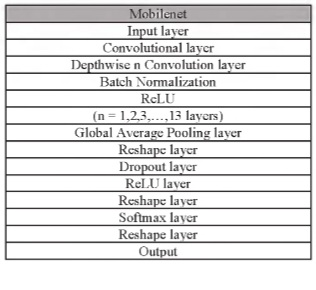
\includegraphics[width=0.7\textwidth]{CNN architecture.jpg}
    \caption{CNN Architecture} 
\end{figure}

\end{frame}

\begin{frame}{Self-driving control architecture}
\begin{block}{Controller}
 \begin{itemize}
     
\item CNN's can be used in place of conventional controllers(CC). 
\item As, CC's may lead to poor handling performances because they need to set up with specific features and hardware parameters.
\item CNN is able to go beyond pattern recognition.It learns the entire processing pipeline needed to steer an automobile.
\item CNN block diagram below is applied to replace the CC's.
\item Furthermore,the CNN can apply on real time processing with or without lane marking.
    \end{itemize}
\end{block}
\end{frame} 
 
 
\begin{frame}    
\begin{figure}[ht]
    \centering
    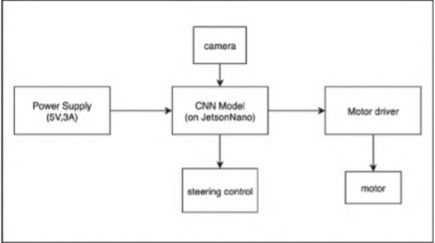
\includegraphics[width=0.8\textwidth]{CNN block diagram.jpg}
    \caption{CNN block diagram}
\end{figure}
\end{frame}

\begin{frame}
 \begin{block}{Hardware optimization}
 A processor with high processing speed and high performance to communicate and respond rapidly is needed in self-driving car(SDC) for driving and steering motor control.
 \begin{enumerate}
     \item The processor for the self-driving car is the Jetson Nano.It is used to compute CNN models .
     \item The controller selected for building SDC is STM32, the main function of controller is communication between the motor drive system and Jetson Nano.
     \item The motor driver chip for building the SDC is L293D.Using this chip can typically power up to 36 volts.
     \item The power supply for SDC is an 11.4 volts 2200mAh Lipo battery.
     all systems in SDC requires power.
 \end{enumerate}
 \end{block}   
\end{frame}

\begin{frame}{Methods and Experiments}
\begin{block}{Experiment Setup}
\begin{itemize}
    \item First, Lipo battery is applied to SDC and set-up an alarm to detect when voltage in each battery cell was lower than threshold.
    \item The steering angle is initially started at 0 degree.
    \end{itemize}
\end{block}


\begin{block}{Data collection}
\begin{itemize}
  \item A data set,captured image and steering angle is collected while controlling the car through a joystick.
  \item Thousands of images are saved into JetsonNano that runs on Ubuntu 14.0 operating system. 
  \item The range of servo motor angle is between -70 to 70 degrees.
\end{itemize}
\end{block}    
\end{frame}

\begin{frame}
\begin{block}{Output data for classification}
\begin{enumerate}
    \item The steering angles collected from a joystick are in between -75 to 75 degrees.
    \item We will segment the steering angle corresponding with image data into five classes.
    \item Below there is fig regarding interval of angles and classes.
    \end{enumerate}
\end{block}
    
\begin{figure}[ht]
    \centering
    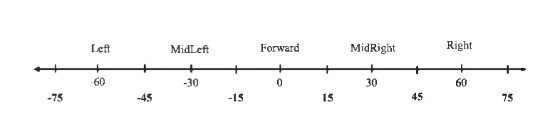
\includegraphics[width=1\textwidth]{SA intervals.jpg}
    \caption{Relation between steering angle and classes} 
    
\end{figure}
    
\end{frame}

\begin{frame}

\begin{block}{Image processing}
  The CNN was designed with $160 \times 160$ pixels for pushing the higher frame rate as fast as possible.The image normalization has been done before applied to the model.
\end{block}

\begin{block}{Data pre processing}
We shuffled data from CSV file that contains the image path and steering angle.The data is divided into training and testing set with ratio of 80\% and 20\% respectively.

\end{block}

\begin{block}{Training model}
\begin{enumerate}

\item When an entire dataset is passed forward or backward through neural network is one epoch.
\item We train the network about 128 epochs. 
\item Accuracy of the training dataset is 94.09\% and the accuracy of the testing dataset is 85.03\%.
\end{enumerate}
\end{block}

\end{frame}

\begin{frame}
\begin{figure}[ht]
    \centering
    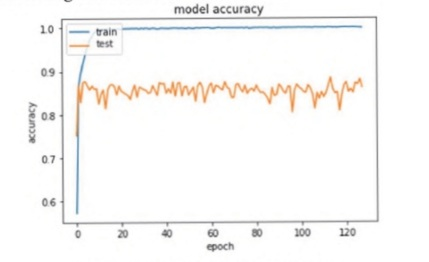
\includegraphics[width=1\textwidth]{Output accuracy.jpg}
    \caption{Output accuracy of 128 epochs diagram}
\end{figure}
    
\end{frame}

\begin{frame}
\begin{block}{Experimental Results}
\begin{itemize}
    \item We test the experiments in 2 phases,software simulation and on road testing.
    \item The CNN model has softmax activation function,the purpose of this activation function is used to predict probability of each classes($P_i$).
    \item In first phase, the images are applied to CNN in order to obtain $P_i$
    corresponding to steering class angle.
    \item The prediction angle from each class is calculated by equation (1).
    \begin{align}
        Angle(degree)=\sum_{i=0}^{4} \brak{P_i \times W_i}
    \end{align}
    where $W_i$ is degrees corresponding to Table 1.
    \item This equation is used to compute output steering angle.
\end{itemize} 
\end{block}
\end{frame}

\begin{frame}
\begin{table}[ht]

\centering
\begin{tabular}{|c|c|c|} \hline
     Class(Probability) & Meaning & Degrees(W_i)  \\ \hline
     Class 0 & Left & -60  \\ \hline
     Class 1 & MidLeft & -30  \\ \hline
     Class 2 & Forward & 0  \\ \hline
     Class 3 & Right & 30  \\ \hline
     Class 4 & MidRight & 60  \\ \hline
\end{tabular}
\caption{1:class meaning and gain for mapping to predicted angle}
\label{1:class meaning and gain for mapping to predicted angle}
\end{table}

\begin{block}{Experimental results}
\begin{itemize}
    \item In second phase,the trained model from the first phase is embedded into car.
    \item The accuracies were calculated from training and phase which are 94.05\% and 85.03\% respectively.
\end{itemize}
\end{block}

\end{frame}

\begin{frame}{Conclusions}
\begin{block}{Conclusions}
\begin{enumerate}
    \item This paper used CNN as a controller.There is no theoretical comparing between using conventional controllers and CNN in SDC.
    \item The conventional ones obtain the errors from measured data while errors in CNN are not directly fed back from output errors. 
    \item CNN is able to learn the the diversified tasks of lanes and the roads following with or without lane marking,direction planning and automatically control.
\end{enumerate}
\end{block}  

\begin{center}
    Thank you!
\end{center}
\end{frame}
\end{document}